\section{Data} \label{sec:data}
From the NeurIPS paper dataset, we remove the papers without abstracts, obtaining 3,924 papers. We then concatenate each paper's abstract with the first 200 tokens of the body text. We split the data into a training set and a test set. The number of papers in each set are described in Table \ref{table:data_stats}.

\begin{figure}
  \centering
    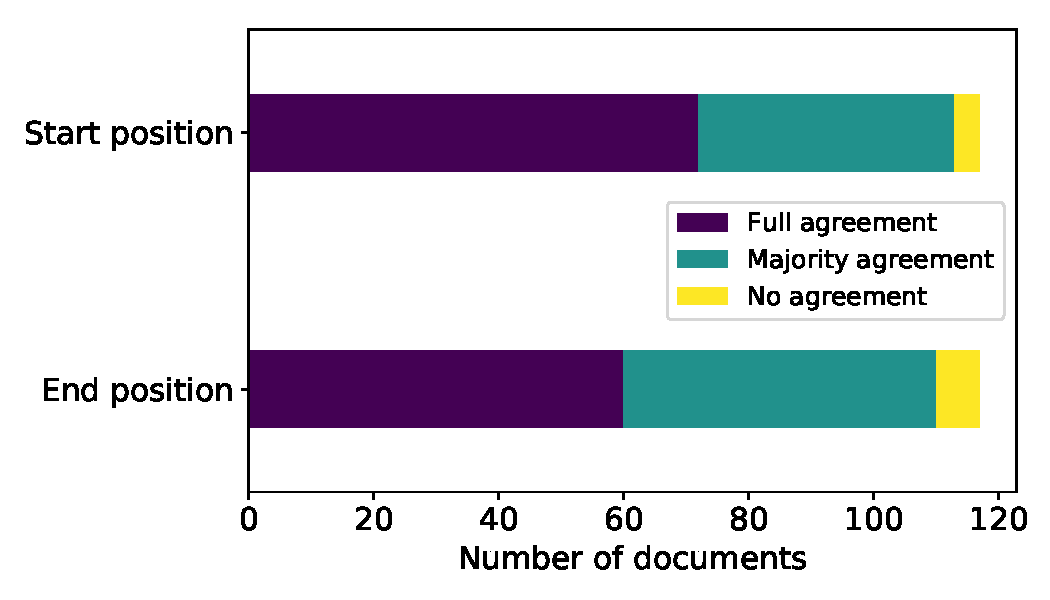
\includegraphics[width=0.5\textwidth]{annotation_agreement.pdf}
      \caption{Agreement on podcast episode introductions with annotation from three annotators. The majority of episodes have a perfect or majority agreement, and few have no agreement.}
    \label{fig:annotation_agreement}
\end{figure}

We collect the podcast transcripts using Google's speech-to-text service. The podcasts are grouped into 20 categories by topic (e.g. news, sports, comedy, etc.). To select data for annotation, we collect 3 recent episodes from the top 10 most popular podcast programs in each category, resulting in a set of 600 episodes. At the time of submission, 417 episodes have been annotated. We only keep the English podcasts and use the original transcriptions without any post-editing.

While the formats of podcasts vary, the episodes in a podcast program usually share similar topic(s) and format(s). For example, all episodes in the \emph{B\&H Photography Podcast}\footnote{\text{https://www.bhphotovideo.com/explora/podcasts}}
are about photography. All episodes in the \emph{Song Exploder}\footnote{\text{http://songexploder.net/}}
program share a similar structure: introduction, a song, and then an interview with the creator(s) of the song. Intuitively, it will be much easier for a model to perform well on given episodes if it is trained on other episodes in the same program. We therefore stratify the data, leaving 5\% of the programs out and use all episodes in these programs as ``test set of unseen programs". From the rest of programs, we further keep 10\% of their episodes as ``test set of seen programs". The rest of the dataset is used as training set. The number of episodes in the training and test sets are summarized in Table \ref{table:data_stats}.

% This allows us to control for the topics and enabling our model to learn the structural segmentation boundaries, while covering a wide variety of data to improve the extensibility of the model. 

\begin{table*}[h]
\centering
\begin{tabular}{llc}
\hline &  \textbf{Training set size} & \textbf{Test set size} \\ \hline
NeurIPS papers & 3531  & 393 \\
Podcast transcripts & 350  & 39 (seen programs)/28 (unseen programs) \\
\hline
\end{tabular}
\caption{ \label{table:data_stats} Number of documents in the training and test sets.}
\end{table*}


A group of 16 annotators were recruited to label the podcast transcripts. Each annotator listens to a podcast episode while looking at its transcript. Annotators are instructed to identify two types of introductions: the first is the \emph{program introduction}---the high-level description of a podcast program's contents, which can be similar or even identical for all episodes in a program. Second, the \emph{episode introduction}, which is a short description of a specific episode's topic, host, guest, or other important subjects discussed in it.  As the program introductions are trivial to identify, we focus on the episode introductions\footnote{Except in this paragraph, we use the word ``introductions" to indicate episode introductions in this paper.}. 

We ask the annotators to label the starting and ending words of each of these contents, or mark ``none" if they are not present. The annotators are also provided with a text box to write their comments. We do not provide a detailed guideline of what is required for an introduction, but encourage the annotators to use their own judgement in order to obtain more spontaneous reaction to the data.

The noisy and error-prone transcripts obtained from ASR data make this task challenging. When the exact beginning or ending word is mis-transcribed, an annotator may have trouble identifying them. Moreover, the time stamps of words are sometimes erroneous, making it impossible to label the exact word. Even if the transcription is perfect, two human annotators may disagree on what constitutes an introduction. Taking account of these issues, we have a number of episodes labeled by three independent annotators. At the time of submission, 117 our of the 417 total episodes have been labeled by three annotators. We define the gold standard to be majority agreement---where at least two out of three annotators have an agreement. If all three annotators agree, we consider it a perfect agreement. Because of the noise in the data, if two labels differ by less than 2 seconds, we consider them as having an agreement. 

We examine the annotator agreement on the 117 episodes with three annotations. Figure \ref{fig:annotation_agreement} shows the number of perfect and majority agreements for these episodes. For the annotations on the start of introductions, out of the 117 episodes, 72 have perfect agreement---i.e. all annotators agree on the same start position. Forty-one episodes have majority agreement, and only 4 have no agreement. If we only consider episodes with perfect or majority agreement, we obtain 113 episodes or 96.6\% of the data. Similarly, considering also the agreement on the end position, we are left with 110 episodes or 94.0\% of the data. For the podcast programs with 100\% annotator agreement, we include all episodes in these programs in the dataset even if they have not been labeled by three independent annotators.

% We also consider the accuracy of annotators by comparing each of their annotations with the gold standard. We find the average accuracy of annotators to be 91.9\%, which we use as the standard for human performance. 



\begin{figure}[ht!]
  \centering
  \vspace{-0.4cm}
    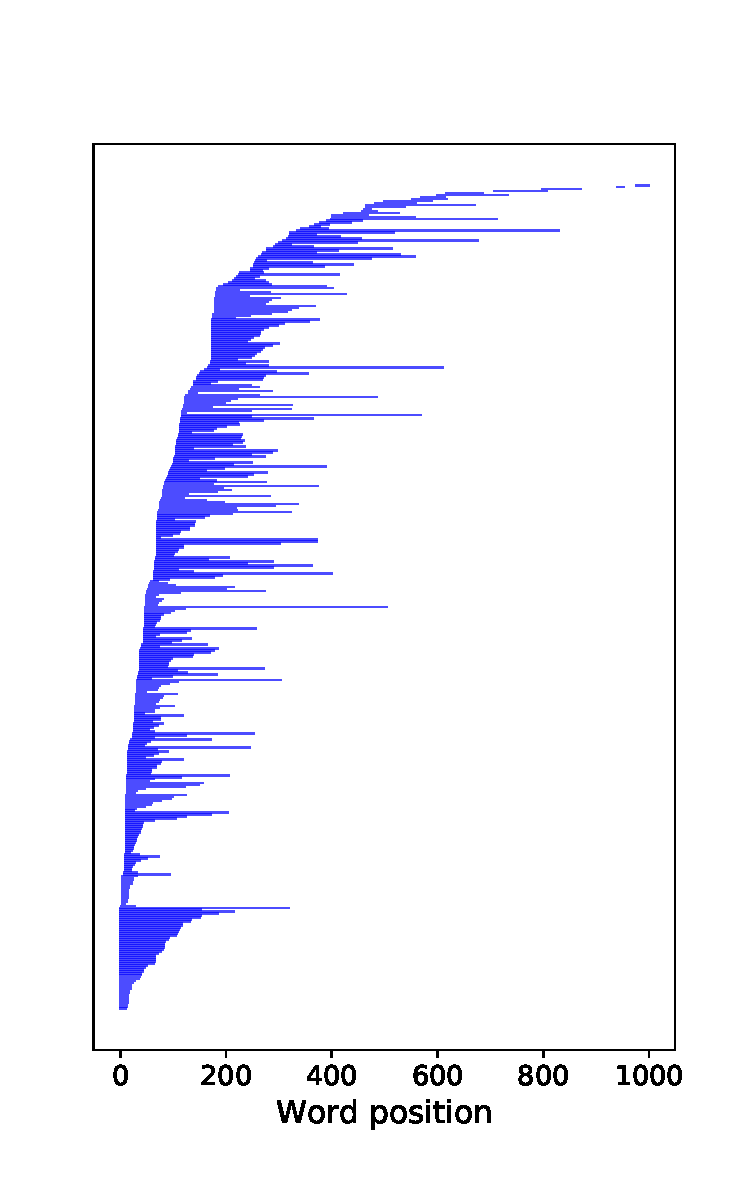
\includegraphics[width=0.5\textwidth]{start_end_position.pdf}
    \vspace{-1cm}
      \caption{Locations of episode introductions in the transcripts. Each line shows the start, end, and duration of an episode's introduction by word positions.}
    \label{fig:start_end_position}
\end{figure}


From the annotated data, we notice that the structures of podcast episodes are not consistent. For example, some episodes have program introductions before episode introductions, and vice versa. A number of episodes do not have any introductions at all. Music and advertisements may also be inserted before or after the introductions. Figure \ref{fig:start_end_position} shows the locations of episode introductions. We found these locations to vary widely, with episode introductions starting or ending as late as near 1,000 words into the transcripts.

